\documentclass{article}
\usepackage[utf8]{inputenc}
\usepackage{amsmath,amsfonts,amssymb,amsthm,mathtools}
\usepackage{parskip}
\usepackage{graphicx}
\usepackage[dvipsnames]{xcolor}

\newcommand{\dd}[2][]{\frac{\partial #1}{\partial #2}}
\newcommand{\dt}[2][]{\frac{d #1}{d #2}}
\renewcommand{\a}{\mathbf{a}}
\newcommand{\A}{\mathbf{A}}
\newcommand{\B}{\mathbf{B}}
\newcommand{\C}{\mathbf{C}}
\newcommand{\I}{\mathbf{I}}

\renewcommand{\b}{\mathbf{b}}
\renewcommand{\L}{\mathcal{L}}

\newcommand{\X}{\mathbf{X}}
\newcommand{\y}{\mathbf{y}}
\newcommand{\w}{\mathbf{w}}

\newtheorem{exercise}{Exercise}
\newtheorem{answer}{Answer}

\title{EMAT31530: Mathematical preliminaries}
\author{Laurence Aitchison}
\date{}

\begin{document}

\maketitle

Here, I'm going to introduce all the mathematical preliminaries and notation that I'm going to use, with a view to their later use in AI.  This was originally designed for CS students, rather than the more Math-y cohort in the course. So you've probably seen the early stuff, but not necessarily the later stuff.  The emphasis might be quite different from stuff you've seen before (as I'm developing stuff necessary for AI).  Everything here is examinable, so please do at least skim through.  And in any case, you really have a go at the should do the exercises (especially the last ones): they're great preparation for later lectures.

\section{Calculus}

AI is all about calculus.  PyTorch is --- in a very literal sense --- one big calculus engine.

\subsection{Polynomials}

The derivative of $x^p$, where $p$ is some power,
\begin{align}
  \dt[x^p]{x} &= p x^{p-1}.
\end{align}
Perhaps the most important example (which we're going to encounter many times) is the derivative of a quadratic,
\begin{align}
  \dt[x^2]{x} &= 2 x.
\end{align}
But the formula also applies for higher powers,
\begin{align}
  \dt[x^5]{x} &= 5 x^4.
\end{align}
And for negative powers,
\begin{align}
  \dt[x^{-3}]{x} &= -3 x^{-4}.
\end{align}
And for fractional powers,
\begin{align}
  \dt[\sqrt{x}]{x} = \dt[x^{1/2}]{x} &= \frac{1}{2} x^{-1/2} =\frac{1}{2 \sqrt{x}}.
\end{align}
And for powers of zero,
\begin{align}
  \dt[1]{x} = \dt[x^0]{x} &= 0 x^{-1} = 0.
\end{align}
(note that $x^0 = 1$, a constant, so the gradient has to be zero).
And for powers of one,
\begin{align}
  \dt[x]{x} = \dt[x^1]{x} &= 1 x^0 = 1.
\end{align}
(note that $x^1 = x$, which has a slope of $1$).
We can apply the rule to each term in a polynomial,
\begin{align}
  \dt{x}[3 x^4 + 2 x^{-1/2} + x^{-2}] &=
  3 \dt[x^4]{x} + 2 \dt[x^{-1/2}]{x} + \dt[x^{-2}]{x}\\
  \intertext{Looking at each term separately,}
  \dt[x^4]{x} &= 4 x^3\\
  \dt[x^{-1/2}]{x} &= -\tfrac{1}{2} x^{-1.5}\\
  \dt[x^{-2}]{x} &= -2 x^{-3}
  \intertext{Putting everything back together,}
  \dt{x}[3 x^4 + 2 x^{-1/2} + x^{-2}] 
  &= 3 (4 x^3) + 2 (-\tfrac{1}{2} x^{1.5}) - 2 x^{-3}\\
  &= 12 x^3 - x^{1.5} - 2 x^{-3}.
\end{align}

\subsection{Chain rule}
To differentiate more complex expressions, we need the chain rule.
For instance, we might have,
\begin{align}
  &\dt[y]{x} &&\text{where} & y(x) &= (x+1)^3
\end{align}
We could expand the brackets, but we don't want to because that would be alot of terms.
Instead, we rewrite $y$ in terms of $u$,
\begin{align}
  u &= x+1 & y &= u^3
\end{align}
Then, we use the chain rule,
\begin{align}
  \dt[y]{x} &= \dt[y]{u} \dt[u]{x}.
\end{align}
And each of these derivatives is much easier,
\begin{align}
  \dt[y]{u} &= \dt[u^3]{u} = 3 u^2\\
  \dt[u]{x} &= \dt[x+1]{x} = \dt[x]{x} + \dt[1]{x} = 1 + 0 = 1
\end{align}
Subsituting these derivatives into the chain rule, we get our answer,
\begin{align}
  \dt[y]{x} &= \dt[y]{u} \dt[u]{x} = 3 u^2 \times 1\\ 
  \intertext{And finally substituting $u=x+1$,}
  \dt[y]{x} &= 3 (x+1)^2.
\end{align}
Despite its simplicity in this example, it turns out that the chain rule is the basis of backprop, and backprop is the basis of all modern AI, from ChatGPT to Stable Diffusion to just about everything else.
This is because the chain rule allows you to ``chain'' together derivatives in a complex, multi-step pipeline.
But that's for later.

\subsection{Product rule}
The final key rule of calculus is the product rule,
\begin{align}
  \dt[u(x) v(x)]{x} &= u(x) \dt[v(x)]{x} + v(x) \dt[u(x)]{x}.
\end{align}
Again, this rule can be used to avoid an explosion of terms.
For instance,
\begin{align}
  y &= (x+x^2+x^3)(2x+3x^2+x^3)
\end{align}
has 9 terms and is really painful to work with.
Instead, if we set,
\begin{align}
  u(x) &= x+x^2+x^3 \\
  v(x) &= 2x+3x^2+x^3
  \intertext{We get,}
  y = u(x) v(x).
\end{align}
Now, we can use the product rule!
\begin{align}
  \dt[y]{x} &= \dt[u(x) v(x)]{x}\\
  &= u(x) \dt[v(x)]{x} + v(x) \dt[u(x)]{x}\\
  &= (x+x^2+x^3) \dt{x}[2x+3x^2+x^3] + (2x+3x^2+x^3) \dt{x}[x+x^2+x^3]\\
  &= (x+x^2+x^3) (2 + 6 x + 3 x^2) + (2x+3x^2+x^3) (1 + 2x + 3x^2)
\end{align}

\subsection{Using calculus to do analytic optimization}
At the top, we mentioned that we were going to use calculus to find e.g.\ the best fitting model (e.g. straight line) to some data.
The starting point is to find a function that measures how good our model is at fitting the data.
Typically, our model has some tunable parameters (e.g.\ the slope of a straight line, which we're going to call $a$).
Then, we have a ``loss'' function $\L(a)$, which takes our tunable parameters as input, and tells us how well the corresponding model fits the data; small values indicate a good fit, and bad values indicate a bad fit.
Typically, the loss function is defined in terms of a \textit{distance}, e.g.\ the distance between our predictions and the data (we'll see this in more depth later).

For the moment, our question is how to find the best model, i.e.\ the value of $a$ with the smallest loss, $\L(a)$.
Well, this is an optimization problem, and it turns out we can use calculus to solve optimization problems.

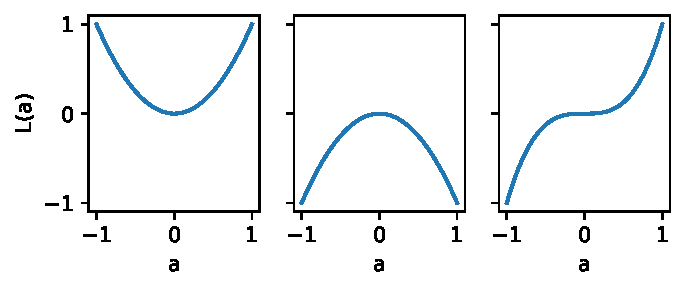
\includegraphics{x2x3.pdf}

Usually, in AI, we find the optimum by gradient descent: following the gradient down hill until you reach a minimum.
But in simple settings, we can solve for the minimum analytically: the minimum of the loss is usually at a location where the gradient is zero (left).  Of course, we have to be careful with this: the gradient can also be zero at a maximum (middle), or at neither a maximum or minmum (right).
Though issues caused by this are very rare, and AI people generally ignore these possibilities.

For instance, the loss might be as simple as a quadratic,
\begin{align}
  \L(a) &= a^2 + 5a - 3
\end{align}
To minimize $\L(a)$, we find the place where the slope is zero,
\begin{align}
  0 &= \dt[\L(a)]{a} \\
  0 &= \dt{a}[a^2 + 5a - 3]\\
  0 &= \dt[a^2]{a} + \dt[5a]{a} - \dt[3]{a}\\
  0 &= 2 a + 5
\end{align}
Then, we can solve for $a$,
\begin{align}
  2a &= -5,\\
  a &= -\tfrac{5}{2}.
\end{align}
Now, this looks kind-of simplistic.
Of course, the real calculation is more complicated, largely because it involves summing over datapoints (which we will see next).
But finding the best model/straight line really does end up involving minimizing a quadratic!

\section{Sums and products}
Typically, we're going to be working $N$ datapoints, where the $i$th datapoint is $x_i$.
So the first datapoint is $x_1$, the second datapoint is $x_2$, and the last datapoint is $x_N$.
We're often going to need to sum or multiply across many different datapoints, similarly to a for loop.

To sum over datapoints, we use the summation notation.  For instance, the sum of $i^2$ for $i=1$ to $i=3$ can be written,
\begin{align}
  \sum_{i=1}^3 i^2 = 1^2 + 2^2 + 3^2.
\end{align}
If we have datapoints, $x_i$, then we could sum over datapoints using,
\begin{align}
  \sum_{i=1}^N x_i = x_1 + x_2 + \dotsm + x_N,
\end{align}
which indicates that we should sum $x_i$ for $i=1$ to $i=N$.

To take a product over datapoints, we use product (or capital pi) notation.  This is just like the sum, except that we multiply each term, rather than adding them.
For instance, the product of $i$ for $i=1$ to $i=3$ can be written,
\begin{align}
  \prod_{i=1}^3 i = 1 \times 2 \times 3.
\end{align}
We could also take the product over datapoints, $x_i$, using,
\begin{align}
  \prod_{i=1}^N x_i = x_1 \times x_2 \times \dotsm \times x_N,
\end{align}
which indicates that we should take the product of $x_i$ for $i=1$ to $i=N$.

I will generally try to be explicit about the upper and lower limits.
But sometimes, especially in other people's material, you will see abbreviated notation, missing off the upper and lower limits.
If the limits are left off, then there should be some ``natural'' values for them to take on.
For instance, if we know that there are $N$ datapoints ranging from $x_1$ to $x_N$, then ``natural'' lower limit is $i=1$ and the ``natural'' upper limit is $i=N$.
\begin{align}
  \sum_i x_i &= \sum_{i=1}^N x_i & \prod_i x_i &= \prod_{i=1}^N x_i
\end{align}
Of course this is context dependent.  The natural limits here are $i=1$ to $i=N$ only because this we knew we had $N$ datapoints.

\section{Logarithms}
Here, $\log$ is \textit{always} the natural logarithm, i.e.\
\begin{align}
  x &= e^{\log x} & x &= \log(e^x).
\end{align}
(and this is also true in numerical programming e.g.\ Python, PyTorch etc.)
For our purposes, the logarithm is super-useful because it converts products into sums,
\begin{align}
  \log(b\times c) &= \log b + \log c.
\end{align}
This extends to powers,
\begin{align}
  \log(x^y) &= \log \underbrace{(x \times x \times \dotsm \times x)}_{y \text{ times}}\\ 
  &= \underbrace{\log x + \log x + \dotsm + \log x}_{y \text { times}}\\
  &= y \log x.
\end{align}
But most importantly, it extends to products and summations over many elements,
\begin{align}
  \log(\prod_{i=1}^N x_i) &= \sum_{i=1}^N \log x_i
\end{align}
Using logs to switch products to sums is going to be important for two reasons:
\begin{itemize}
  \item its much easier to do e.g.\ calculus on sums than on products.
  \item If you have a big product, the result might lie outside the range of float32/float64.  The minimum value of float32 is $1.2\times10^{-38}$.  If we have $x_i=0.1$ and $N$ = 38, then $\prod_{i=1}^N x_i = 10^{-38}$, and we're only just inside the range of float32's.
\end{itemize}

\section{Vectors, matrices and index notation}

\subsection{Notation/types}

To be super-clear about everything's type, we always ensure scalars/vectors/matrices are distinguishable.  In particular, we always write:
\begin{itemize}
  \item Scalars as non-bold (e.g.\ $a$ or $A$).
  \item Vectors as bold and lowercase (e.g.\ $\a$).  (Single-underline when handwritten.)
  \item Matrices as bold and uppercase (e.g.\ $\A$).  (Double-underline when handwritten.)
\end{itemize}

\renewcommand{\r}{\mathbf{r}}
\renewcommand{\c}{\mathbf{c}}
Unfortunately, vectors can be row \textit{or} column vectors, depending on context.
This ambiguity is PyTorch / Python's fault.  But we can't really do anything about it.
The components of the row-vector $\r$ and column-vector $\c$ can be written,
\begin{align}
  \c &= \begin{pmatrix} c_1 \\ c_2 \\ \vdots \\ c_N \end{pmatrix} &
  \r &= \begin{pmatrix} r_1 & r_2 & \hdots & r_N \end{pmatrix} 
\end{align}
Here, $c_i$ or $r_i$ is a single component of the vector.
Note that elements of vectors/matrices, here $c_i$ or $r_i$, are always scalars, so they are always non-bold.

\newcommand{\N}{\textcolor{red}{N}}
\newcommand{\M}{\textcolor{blue}{M}}
\newcommand{\row}{\textcolor{red}{row}}
\newcommand{\column}{\textcolor{blue}{column}}
\newcommand{\rows}{\textcolor{red}{rows}}
\newcommand{\columns}{\textcolor{blue}{columns}}
\renewcommand{\i}{\textcolor{red}{i}}
\renewcommand{\j}{\textcolor{blue}{j}}
We write matrices as bold upper-case letters, such as $\A$.
A single component of $\A$ is a scalar, so it written non-bold, as $A_{\i\j}$, where $\i$ indexes the \row{} and $\j$ indexes the \column{}.
We write the shape as $\N \times \M$, which means it has $\N$ \rows{} and $\M$ \columns{}.
\begin{itemize}
  \item $\i$ indexes \rows{} and we have $\N$ \rows{}, so $\i$ runs from $1$ to $\N$.
  \item $\j$ indexes \columns{} and we have $\M$ \columns{}, so $\j$ runs from $1$ to $\M$.
\end{itemize}
Remember that we write $\N$ first in $\N \times \M$, and $\i$ is the first index in $A_{\i\j}$, so it is $\i$ that runs from $1$ to $\N$.

Dropping the colours, an $N \times M$ matrix $\A$, can be written,
\begin{align}
  \A &= \begin{pmatrix} 
    a_{11} & a_{12} & \hdots & a_{1\M}\\
    a_{21} & a_{22} & \hdots & a_{2\M}\\
    \vdots & \vdots & \ddots & \vdots\\
    a_{\N1} & a_{\N2} & \hdots & a_{\N\M}.
  \end{pmatrix},
\end{align}
Note how the first index maxes out in the last row at $\N$ and the second index maxes out in the last column at $\M$.

\subsection{Vectors as matrices with one row/column}
Its going to be useful when we come to transposes and matrix products to think of a vector as a matrix with either one row or one column.

A column vector $\c$ with length $N$, can be written,
\begin{align}
  \c &= \begin{pmatrix} c_1 \\ c_2 \\ \vdots \\ c_N \end{pmatrix},
\end{align}
and can be understood as an $N\times 1$ matrix.

A row vector, $\r$ with length $M$, can be written,
\begin{align}
  \r &= \begin{pmatrix} r_1 & r_2 & \hdots & r_M \end{pmatrix}.
\end{align}
and can be understood as an $1\times M$ matrix.


\subsection{Transposes}
The transpose ``mirrors'' the matrix or vector along the diagonal.
For instance, transpose converts the $N \times 1$ column vector $\c$ into a $1 \times N$ row vector, $\c^T$,
\begin{align}
  \c &= \begin{pmatrix} c_1 \\ c_2 \\ \vdots \\ c_N \end{pmatrix} & 
  \c^T &= \begin{pmatrix} c_1 & c_2 & \hdots & c_N \end{pmatrix}
\end{align}
Likewise, it converts the $2\times 3$ matrix $\B$, into the $3 \times 2$ matrix $\B^T$,
\begin{align}
  \B &= \begin{pmatrix}
    1 & 2 & 3 \\ 
    4 & 5 & 6
  \end{pmatrix} & 
  \B^T &= \begin{pmatrix}
    1 & 4 \\
    2 & 5 \\
    3 & 6
  \end{pmatrix}
\end{align}

\subsection{Matrix-matrix product}
\renewcommand{\M}{\textcolor{red}{M}}
\renewcommand{\N}{\textcolor{OliveGreen}{N}}
\renewcommand{\P}{\textcolor{blue}{P}}
\renewcommand{\i}{\textcolor{red}{i}}
\renewcommand{\j}{\textcolor{OliveGreen}{j}}
\renewcommand{\k}{\textcolor{blue}{k}}
The matrix product is just a very short notation for writing a sum and a product.
Before delving into the exact definition, its worth thinking about the matrix sizes. For the product of $\A$ and $\B$,
\begin{align}
  \underbrace{\C}_{\textcolor{red}{M} \times \textcolor{blue}{P}} &= \underbrace{\A}_{\textcolor{red}{M} \times \N} \underbrace{\B}_{\N \times \textcolor{blue}{P}}.
\end{align}
In particular: 
\begin{itemize}
  \item the two inner dimensions, $\N$, must be the same size and they're going to disappear (these are the dimensions we're going to sum over).
  \item $\C$ and $\A$ have the same number of rows, $\M$ (first).
  \item $\C$ and $\B$ have the same number of columns, $\P$ (second).
\end{itemize}
Now lets delve in to the exact definition as a sum and product,
\begin{align}
  C_{\i\k} &= \sum_{\j=1}^{\N} A_{\i\j} B_{\j\k}.
\end{align}
We've highlighted the indices in the same colors as above. 
You can see that the structure of the indices matches that of the sizes above.
In particular: 
\begin{itemize}
  \item we sum over the inner two indices, $\j$ (i.e.\ the second index of $\A$ and the first index of $\B$.
  \item $\i$ is the first index of $\A$ and $\C$ (rows).
  \item $\k$ is the second index of $\B$ and $\C$ (columns).
\end{itemize}

\subsubsection{Matrix multiplication by hand}

To actually do the matrix multiplication, you can use the ``two finger method''.
You move your left finger left-to-right along a row on the first matrix, and your right finger top-to-bottom down a column on the second matrix.
You then multiply the first two elements you see, and add them to your running total.
You choose the row and column based on the element you're trying to calculate.
If you're trying to calculate the element in the second row and the third column, then you'd run your left finger along the second row and you'd run your right finger down the third column.
\begin{align}
  \begin{pmatrix}
    r_{11} & \\
      &
  \end{pmatrix} &= 
  \begin{pmatrix}
  \rightarrow & \rightarrow \\
              &
  \end{pmatrix}
  \begin{pmatrix}
    \downarrow & \\
    \downarrow &
  \end{pmatrix}
\end{align}

\begin{align}
  \begin{pmatrix}
      & r_{12}\\
      &
  \end{pmatrix} &= 
  \begin{pmatrix}
  \rightarrow & \rightarrow \\
              &
  \end{pmatrix}
  \begin{pmatrix}
    & \downarrow \\
    & \downarrow 
  \end{pmatrix}
\end{align}

\begin{align}
  \begin{pmatrix}
      & \\
    r_{21} &
  \end{pmatrix} &= 
  \begin{pmatrix}
  & \\
   \rightarrow & \rightarrow 
  \end{pmatrix}
  \begin{pmatrix}
    \downarrow & \\
    \downarrow & 
  \end{pmatrix}
\end{align}

\begin{align}
  \begin{pmatrix}
      & \\
      & r_{22}
  \end{pmatrix} &= 
  \begin{pmatrix}
  & \\
   \rightarrow & \rightarrow 
  \end{pmatrix}
  \begin{pmatrix}
    & \downarrow \\
    & \downarrow 
  \end{pmatrix}
\end{align}

\subsubsection{Matrix multiplication example}
You can verify the first line by using the ``two-finger method'' described above, or by using the explicit formula for matrix multiplication.
\begin{align}
  \begin{pmatrix}
    5 & 6 \\
    7 & 8
  \end{pmatrix}
  \begin{pmatrix}
    1 & 2 \\
    3 & 4
  \end{pmatrix}
  &= 
  \begin{pmatrix}
    5 \times 1 + 6 \times 3 & 5 \times 2 + 6 \times 4\\
    7 \times 1 + 8 \times 3 & 7 \times 2 + 8 \times 4
  \end{pmatrix}\\
  &= 
  \begin{pmatrix}
    5 + 18 & 10 + 24\\
    7 + 24 & 14 + 32
  \end{pmatrix}\\
  &=
  \begin{pmatrix}
    23 & 34\\
    31 & 46
  \end{pmatrix}
\end{align}


%TODO: Matrix example?

\subsection{Matrix-vector product}
A matrix-vector product is the same as the matrix-matrix product, but we take $\P=1$.
That gives sizes,
\begin{align}
  \underbrace{\mathbf{v}}_{\M \times 1} &= \underbrace{\A}_{\M \times \N} \underbrace{\c}_{\N \times 1}
\end{align}
where both $\mathbf{v}$ and $\c$ are column-vectors.
The exact form for the summation is usually written a bit differently, omitting $\k$ because there's only one possible value for $\k$,
\begin{align}
  v_{\i} &= \sum_{\j=1}^{\N} A_{\i\j} c_{\j}.
\end{align}

\subsection{Vector-matrix product}
A vector-matrix product is the same as the matrix-matrix product, but we take $\M=1$.
That gives sizes,
\begin{align}
  \underbrace{\mathbf{v}}_{1 \times \P} &= \underbrace{\r}_{1 \times \N} \underbrace{\B}_{\N \times \P}
\end{align}
where both $\mathbf{v}$ and $\r$ are row-vectors.
The exact form for the summation is usually written a bit differently, omitting $\i$ because there's only one possible value for $\i$,
\begin{align}
  v_{\k} &= \sum_{\j=1}^{\N} r_{\j} A_{\j\k}
\end{align}

\subsection{Vector inner product}
A vector inner product is the same as the matrix-matrix product, but we take $\M=1$ and $\P=1$, so the output is scalar.
For a vector inner product, the first argument needs to be a row-vector, and the second argument needs to be a column-vector,
\begin{align}
  \underbrace{v}_{1 \times 1} &= \underbrace{\r}_{1 \times \N} \underbrace{\c}_{\N \times 1}\\
\end{align}
where remember $\r$ is a row-vector,  $\c$ is a column-vector, and $v$ is a scalar (or a $1\times 1$ matrix).
We write the summation for omitting $\i$ and $\k$,
\begin{align}
  c &= \sum_{\j=1}^{\N} r_{\j} c_{\j}.
\end{align}
Using transposes, we can also use the vector inner product to combine a column matrix with itself, or a row matrix with itself,
\begin{align}
  \underbrace{v}_{1 \times 1} &= \underbrace{\c^T}_{1 \times \N} \underbrace{\c}_{\N \times 1} & 
  \underbrace{v}_{1 \times 1} &= \underbrace{\r}_{1 \times \M} \underbrace{\r^T}_{\M \times 1}
\end{align}

\subsection{Vector outer product}
A vector-vector product is the same as the matrix-matrix product, but we take $\N=1$, so the output is a matrix.
For a vector inner product, the first argument needs to be a column-vector, and the second argument needs to be a row-vector,
\begin{align}
  \underbrace{\mathbf{V}}_{\M \times \P} &= \underbrace{\c}_{\M \times 1} \underbrace{\b^T}_{1 \times \P}
\end{align}
where remember $\c$ is a column-vector, $\r$ is a row-vector, and $\mathbf{V}$ is a matrix.
We can write the outer product in index notation as,
\begin{align}
  C_{\i,\k} &= a_{\i} b_{\k}.
\end{align}
Using transposes, we can also use the vector outer product to combine a column matrix with itself, or a row matrix with itself,
\begin{align}
  \underbrace{\mathbf{V}}_{\N \times \N} &= \underbrace{\c}_{\N \times 1} \underbrace{\c^T}_{1 \times \N} & 
  \underbrace{\mathbf{V}}_{\M \times \M} &= \underbrace{\r^T}_{\M \times 1} \underbrace{\r}_{1 \times \M} 
\end{align}

\subsection{Identity matrix}
The identity matrix has ones along the diagonal, and zero elsewhere,
\begin{align}
  \I &= \begin{pmatrix}
    1 & 0 \\
    0 & 1 \\
  \end{pmatrix}
\end{align}
If we multiply the identity matrix by any vector / matrix, we just get back the same thing,
\begin{align}
  \I \C &= \C \\
  \C \I &= \C \\
  \r \I &= \r \\
  \I \c &= \c
\end{align}

\subsection{Matrix inverse}
The inverse, $\A^{-1}$, of a matrix, $\A$ is the matrix such that,
\begin{align}
  \I &= \A^{-1} \A
\end{align}
In the $2\times 2$ case,
\begin{align}
  \A &= \begin{pmatrix}
    a & b \\
    c & d \\
  \end{pmatrix} &
  \A^{-1} &= \frac{1}{ad-bc} \begin{pmatrix}
    d & -b \\
    -c & a \\
  \end{pmatrix}
\end{align}
We can prove that this holds by first substituting the value of $\A$ and $\A^{-1}$,
\begin{align}
    \A^{-1} \A &= \frac{1}{ad-bc} \begin{pmatrix}
    d & -b \\
    -c & a \\
  \end{pmatrix}
  \begin{pmatrix}
    a & b \\
    c & d \\
  \end{pmatrix}\\
  \intertext{Then we use the expression for matrix multiplication,}
  \A^{-1} \A &= \frac{1}{ad-bc} \begin{pmatrix}
    ad - bc & db - bd \\
    -ca + ac & ad - bc
  \end{pmatrix}\\
  \A^{-1} \A &= \frac{1}{ad-bc} \begin{pmatrix}
    ad - bc & 0 \\
    0 & ad - bc
  \end{pmatrix}\\
  \A^{-1} \A &= \begin{pmatrix}
    1 & 0 \\
    0 & 1 \\
  \end{pmatrix} = \I
\end{align}
In the ``real-world'', we use the computer to compute our matrix inverses.

\section{Kronecker delta}
The Kronecker delta, $\delta_{ij}$ appears when we start differentiating sums / vectors /matrices.
Its a bit like the indices of an identity matrix (except that we never write $I_{ij}$,
\begin{align}
  \delta_{ij} = \begin{cases}
    1 & \text{if } i=j\\
    0 & \text{otherwise}
  \end{cases}
\end{align}.

\subsection{The Kronecker delta often appears when we're taking gradients of vectors}
Consider a vector,
\begin{align}
  \a^T = \begin{pmatrix}
    a_1 & a_2 & a_3
  \end{pmatrix}
\end{align}
One thing we might want to do (usually as part of a larger calculation) is compute the gradient of $\a$ wrt one of the components, $a_1$,
\begin{align}
  \dt[\a^T]{a_2} &= \begin{pmatrix}
    \dt[a_1]{a_2} & \dt[a_2]{a_2} & \dt[a_3]{a_2}
  \end{pmatrix}\\
  \intertext{The gradient is zero when the variables don't match, as e.g. changing $a_2$ doesn't cause $a_1$ to change at all,}
  \dt[\a^T]{a_2} &= \begin{pmatrix}
    0 & 1 & 0
  \end{pmatrix}
\end{align}
Now, we can do the same thing a bit more abstractly,
\begin{align}
  \a^T &= \begin{pmatrix}
    a_1 & a_2 & \hdots & a_N
  \end{pmatrix}\\
  \dt[\a^T]{a_j} &= \begin{pmatrix}
    \dt[a_1]{a_j} & \dt[a_2]{a_j} & \hdots & \dt[a_N]{a_j}
  \end{pmatrix}\\
  \intertext{To represent that these gradients are $1$ only when the top index matches the bottom index, we use the Kronecker delta,}
  \dt[\a^T]{a_j} &= \begin{pmatrix}
    \delta_{1j} & \delta_{2j} & \hdots & \delta_{Nj}
  \end{pmatrix}\\
  \intertext{And if we select out the $i$th element of the vector,}
  \dt[a_i]{a_j} &= \delta_{ij}.
\end{align}

\subsection{The Kronecker delta picks out an element of a sum}
You should be happy to see a Kronecker delta turn up, because it typically makes things alot simpler!
In particular, we often have Kronecker deltas in sums, and the Kronecker delta ``picks out'' one element of the sum.
\begin{align}
  \sum_{j=1}^3 \delta_{2 j} a_j &= \delta_{2 1} x_1 + \delta_{2 2} x_2 + \delta_{2 3} x_3 \\
  &= 0 x_1 + 1 x_2 + 0 x_3 \\
  &= x_2.
\end{align}
This notion of ``picking out one element'' is perhaps easier to see in the more general case,
\begin{align}
  \sum_j \delta_{i j} a_j &= a_i,
\end{align}
which happens because $\delta_{ij}$ is zero for all $j$ except when $j=i$.

\clearpage

\section{Exercises}

You can skip the unit exercises if they look straightforward to you.  But please do try the last one!

\begin{exercise}
  Calculate:
  \begin{align}
    \dt{x}[4x^{2.5} + x^{1/2} - 6 x^{-1/2}]
  \end{align}
\end{exercise}

\begin{exercise}
  Use the chain rule to calculate:
  \begin{align}
    \dt{x} [(x+1)^3]
  \end{align}
\end{exercise}

\begin{exercise}
  Calculate the same thing, without using the chain rule, by explicitly expanding the brackets and applying $\dt[x^p]{x} = p x^{p-1}$,
  \begin{align}
    \dt{x} [(x+1)^3]
  \end{align}
  Check they give the same answer!
\end{exercise}

\begin{exercise}
  Find the minimum of,
  \begin{align}
    \L(a) = 4 a^2 + 2 a + 1.
  \end{align}
\end{exercise}

\begin{exercise}
  Calculate,
  \begin{align}
    \sum_{i=0}^5 i^2.
  \end{align}
\end{exercise}

\begin{exercise}
  Calculate,
  \begin{align}
    \prod_{i=1}^5 i.
  \end{align}
\end{exercise}

\begin{exercise}
  Simplify,
  \begin{align}
    \sum_{i=1}^N b
  \end{align}
  where b does not depend on i.
\end{exercise}

\begin{exercise}
  Simplify,
  \begin{align}
    \prod_{i=1}^N b
  \end{align}
  where b does not depend on i.
\end{exercise}

\begin{exercise}
  Compute the matrix product,
  \begin{align}
    \begin{pmatrix}
      1 & 2 \\
      3 & 4
    \end{pmatrix}
    \begin{pmatrix}
      5 & 6 \\
      7 & 8
    \end{pmatrix}
  \end{align}
\end{exercise}

\begin{exercise}
  Compute the matrix inverse,
  \begin{align}
    \begin{pmatrix}
      1 & 2 \\
      3 & 4
    \end{pmatrix}^{-1}
  \end{align}
\end{exercise}

\begin{exercise}
  Use the matrix inverse to solve the following expression for $x_1$ and $x_2$,
  \begin{align}
    \begin{pmatrix}
      1 & 2 \\
      3 & 4
    \end{pmatrix}
    \begin{pmatrix}
      x_1 \\
      x_2
    \end{pmatrix}
    = 
    \begin{pmatrix}
      5 \\ 6
    \end{pmatrix}
  \end{align}
\end{exercise}

\begin{exercise}
  Find the value of 
  \begin{align}
    \dt[y_i]{w_k}
  \end{align}
  in terms of the fixed $\X$, where $\y$ is given by,
  \begin{align}
    \y &= \X \w
  \end{align}
\end{exercise}

\clearpage
\section{Answers}

\begin{answer}
  Calculate:
  \begin{align}
    \dt{x}[4x^{2.5} + x^{1/2} - 6 x^{-1/2}] &= 
    4\dt[x^{2.5}]{x} + \dt[x^{1/2}]{x} - 6 \dt[x^{-1/2}]{x}\\
    &= 4(2.5 x^{1.5}) + \tfrac{1}{2} x^{-1/2} - 6 (-\tfrac{1}{2} x^{-1.5})\\
    &= 10 x^{1.5} + \tfrac{1}{2} x^{-1/2} + 3x^{-1.5})
  \end{align}
\end{answer}

\begin{answer}
  Use the chain rule to calculate:
  \begin{align}
    \dt{x} [(x+1)^3]
    \intertext{set}
    u &= (x+1)\\
    y &= (x+1)^3 = u^3
    \intertext{Thus we can apply the chain rule,}
    \dt{x} [(x+1)^3] &= \dt[y]{x}\\
    &= \dt[u]{x} \dt[y]{u}\\
    &= \dt[x+1]{x} \dt[u^3]{u}\\
    &= 1 \times 3 u^2\\
    &= 3 (x+1)^2
  \end{align}
\end{answer}

\begin{answer}
  Calculate the same thing, without using the chain rule, but explicitly expanding the brackets and applying $\dt[x^p]{x} = p x^{p-1}$,
  \begin{align}
    \dt{x} [(x+1)^3] &= \dt{x}[(x+1) (x+1) (x+1)]\\
    &= \dt{x}[(x^2 + 2 x + 1) (x+1)]\\
    &= \dt{x}[(x^3 + 2 x^2 + x) + (x^2 + 2 x + 1)]\\
    &= \dt{x}[(x^3 + 3 x^2 + 3 x + 1)]\\
    &= 3 x^2 + 6 x + 3\\
    &= 3 (x^2 + 2 x + 1)\\
    &= 3 (x+1)^2
  \end{align}
\end{answer}

\begin{answer}
  Find the minimum of,
  \begin{align}
    \L(a) = 4 a^2 + 2 a + 1.
  \end{align}
  Solve for the value of $a$ where the gradient is zero,
  \begin{align}
    0 &= \dt[\L(a)]{a} \\
    &= \dt{a}[4 a^2 + 2 a + 1]\\
    &= 4 \dt{a}[a^2] + 2 \dt[a]{a} + \dt[1]{a}\\
    &= 4 (2 a) + 2\\
    &= 8 a + 2.
  \end{align}
  Now, we can solve for $a$,
  \begin{align}
    8 a &= -2\\
    a &= -\tfrac{1}{4}.
  \end{align}
\end{answer}

\begin{answer}
  Calculate,
  \begin{align}
    \sum_{i=0}^5 i^2 &= 0^2 + 1^2 + 2^2 + 3^2 + 4^2 + 5^2\\
    &= 0 + 1 + 4 + 9 + 16 + 25\\
    &= 14+16+25\\
    &= 30+25\\
    &= 55
  \end{align}
\end{answer}

\begin{answer}
  Calculate,
  \begin{align}
    \prod_{i=1}^5 i &= 1 \times 2 \times 3 \times 4 \times 5\\
    &= (2 \times 3) \times (4 \times 5)\\
    &= 6 \times 20\\
    &= 120
  \end{align}
\end{answer}

\begin{answer}
  \begin{align}
    \sum_{i=1}^N b &= \underbrace{b + b + \dotsm + b}_{N \text{ times}} = N b
  \end{align}
\end{answer}

\begin{answer}
  \begin{align}
    \prod_{i=1}^N b &= \underbrace{b \times b \times \dotsm \times b}_{N \text{ times}} = b^N
  \end{align}
\end{answer}

\begin{answer}
  \begin{align}
    \begin{pmatrix}
      1 & 2 \\
      3 & 4
    \end{pmatrix}
    \begin{pmatrix}
      5 & 6 \\
      7 & 8
    \end{pmatrix}
    &= 
    \begin{pmatrix}
      1 \times 5 + 2 \times 7 & 1 \times 6 + 2 \times 8\\
      3 \times 5 + 4 \times 7 & 3 \times 6 + 4 \times 8
    \end{pmatrix}\\
    &= 
    \begin{pmatrix}
      5 + 14 & 6 + 16\\
      15 + 28 & 18 + 32
    \end{pmatrix}\\
    &=
    \begin{pmatrix}
      19 & 22\\
      43 & 50
    \end{pmatrix}
  \end{align}
\end{answer}

\begin{answer}
  Matrix inverse:
  \begin{align}
    \begin{pmatrix}
      1 & 2 \\
      3 & 4
    \end{pmatrix}^{-1}
    &= \frac{1}{1\times 4 - 2 \times 3} 
    \begin{pmatrix}
      4 & -2 \\
      -3 & 1
    \end{pmatrix}\\
    &= \frac{1}{4 - 6}
    \begin{pmatrix}
      4 & -2 \\
      -3 & 1
    \end{pmatrix}\\
    &= - \frac{1}{2}
    \begin{pmatrix}
      4 & -2 \\
      -3 & 1
    \end{pmatrix}\\
    &= \frac{1}{2}
    \begin{pmatrix}
      - 4 & 2 \\
      3 & -1
    \end{pmatrix}
  \end{align}
\end{answer}

\begin{answer}
  \begin{align}
    \begin{pmatrix}
      1 & 2 \\
      3 & 4
    \end{pmatrix}
    \begin{pmatrix}
      x_1 \\
      x_2
    \end{pmatrix}
    &= 
    \begin{pmatrix}
      5 \\ 6
    \end{pmatrix}\\
    \intertext{Multiply on both sides by the inverse of the matrix,}
    \begin{pmatrix}
      1 & 2 \\
      3 & 4
    \end{pmatrix}^{-1}
    \begin{pmatrix}
      1 & 2 \\
      3 & 4
    \end{pmatrix}
    \begin{pmatrix}
      x_1 \\
      x_2
    \end{pmatrix}
    &= 
    \begin{pmatrix}
      1 & 2 \\
      3 & 4
    \end{pmatrix}^{-1}
    \begin{pmatrix}
      5 \\ 6
    \end{pmatrix}\\
    \intertext{A matrix times matrix-inverse is the identity,}
    \begin{pmatrix}
      x_1 \\
      x_2
    \end{pmatrix}
    &= 
    \begin{pmatrix}
      1 & 2 \\
      3 & 4
    \end{pmatrix}^{-1}
    \begin{pmatrix}
      5 \\ 6
    \end{pmatrix}\\
    \intertext{We can substitute for the value of the matrix inverse from the previous question,}
    \begin{pmatrix}
      x_1 \\
      x_2
    \end{pmatrix}
    &= 
    \frac{1}{2}
    \begin{pmatrix}
      - 4 & 2 \\
      3 & -1
    \end{pmatrix}
    \begin{pmatrix}
      5 \\ 6
    \end{pmatrix}\\
    \intertext{Then compute the matrix-vector product,}
    \begin{pmatrix}
      x_1 \\
      x_2
    \end{pmatrix}
    &= 
    \frac{1}{2}
    \begin{pmatrix}
      (-4) \times 5 + 2 \times 6 \\
      3 \times 5 + (-1) \times 6
    \end{pmatrix}\\
    \begin{pmatrix}
      x_1 \\
      x_2
    \end{pmatrix}
    &= 
    \frac{1}{2}
    \begin{pmatrix}
      -20 + 12\\
      15 - 6
    \end{pmatrix}\\
    \begin{pmatrix}
      x_1 \\
      x_2
    \end{pmatrix}
    &= 
    \frac{1}{2}
    \begin{pmatrix}
      -8\\
      9
    \end{pmatrix}.
    \intertext{We can check this value for $x_1$ and $x_2$ is correct by substituting it back in,}
    \begin{pmatrix}
      1 & 2 \\
      3 & 4
    \end{pmatrix}
    \frac{1}{2}
    \begin{pmatrix}
      -8\\
      9
    \end{pmatrix}
    &=
    \frac{1}{2} \begin{pmatrix}
      1 \times (-8) + 2 \times 9 \\
      3 \times (-8) + 4 \times 9
    \end{pmatrix}\\
    &=
    \frac{1}{2} \begin{pmatrix}
      -8 + 18\\
      -24 + 36
    \end{pmatrix}\\
    &=
    \frac{1}{2} \begin{pmatrix}
      10\\
      12
    \end{pmatrix}\\
    &=
    \begin{pmatrix}
      5\\
      6
    \end{pmatrix}
  \end{align}
\end{answer}
So our result was correct!


\begin{answer}
  We can write out $y_i$ index notation,
  \begin{align}
    y_i &= \sum_{j=1}^N X_{ij} w_j
  \end{align}
  Then subsitute this expression for $y_i$ into the gradient we're trying to compute,
  \begin{align}
    \dt[y_i]{w_k} &= \dt{w_k}[\sum_{j=1}^N X_{ij} w_j]
    \intertext{As $X_{ij}$ is constant,}
    \dt[y_i]{w_k} &= \sum_{j=1}^N X_{ij} \dt[w_j]{w_k}
    \intertext{The gradient is one when $j=k$, and zero otherwise, which matches the definition of the Kronecker delta,}
    \dt[y_i]{w_k} &= \sum_{j=1}^N X_{ij} \delta_{jk}.
    \intertext{Remember that the Kronecker delta is $1$ when $j=k$ and zero otherwise, so the Kronecker delta picks out the $j=k$ element of the loop,}
    \dt[y_i]{w_k} &= X_{ik}.
  \end{align}
\end{answer}


\end{document}

